% Created by tikzDevice version 0.10.1 on 2017-10-23 14:30:52
% !TEX encoding = UTF-8 Unicode
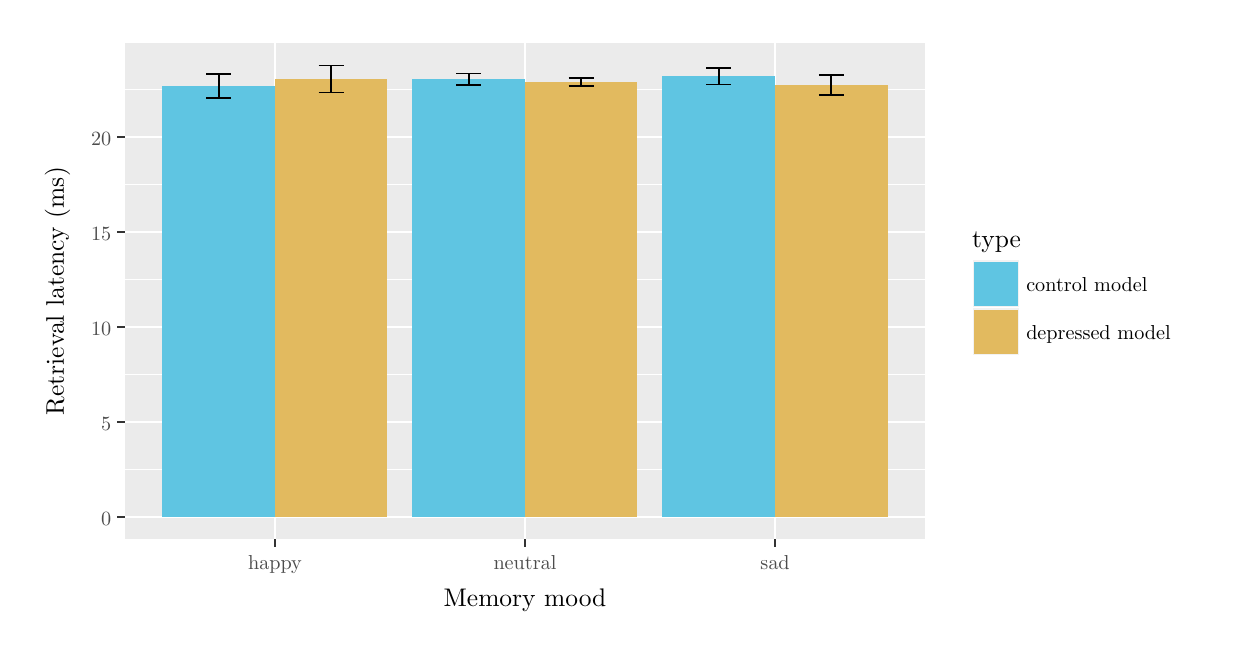
\begin{tikzpicture}[x=1pt,y=1pt]
\definecolor{fillColor}{RGB}{255,255,255}
\path[use as bounding box,fill=fillColor,fill opacity=0.00] (0,0) rectangle (433.62,216.81);
\begin{scope}
\path[clip] (  0.00,  0.00) rectangle (433.62,216.81);
\definecolor{drawColor}{RGB}{255,255,255}
\definecolor{fillColor}{RGB}{255,255,255}

\path[draw=drawColor,line width= 0.6pt,line join=round,line cap=round,fill=fillColor] (  0.00,  0.00) rectangle (433.62,216.81);
\end{scope}
\begin{scope}
\path[clip] ( 35.14, 31.92) rectangle (324.25,211.31);
\definecolor{fillColor}{gray}{0.92}

\path[fill=fillColor] ( 35.14, 31.92) rectangle (324.25,211.31);
\definecolor{drawColor}{RGB}{255,255,255}

\path[draw=drawColor,line width= 0.3pt,line join=round] ( 35.14, 57.22) --
	(324.25, 57.22);

\path[draw=drawColor,line width= 0.3pt,line join=round] ( 35.14, 91.52) --
	(324.25, 91.52);

\path[draw=drawColor,line width= 0.3pt,line join=round] ( 35.14,125.81) --
	(324.25,125.81);

\path[draw=drawColor,line width= 0.3pt,line join=round] ( 35.14,160.11) --
	(324.25,160.11);

\path[draw=drawColor,line width= 0.3pt,line join=round] ( 35.14,194.40) --
	(324.25,194.40);

\path[draw=drawColor,line width= 0.6pt,line join=round] ( 35.14, 40.07) --
	(324.25, 40.07);

\path[draw=drawColor,line width= 0.6pt,line join=round] ( 35.14, 74.37) --
	(324.25, 74.37);

\path[draw=drawColor,line width= 0.6pt,line join=round] ( 35.14,108.66) --
	(324.25,108.66);

\path[draw=drawColor,line width= 0.6pt,line join=round] ( 35.14,142.96) --
	(324.25,142.96);

\path[draw=drawColor,line width= 0.6pt,line join=round] ( 35.14,177.25) --
	(324.25,177.25);

\path[draw=drawColor,line width= 0.6pt,line join=round] ( 89.35, 31.92) --
	( 89.35,211.31);

\path[draw=drawColor,line width= 0.6pt,line join=round] (179.70, 31.92) --
	(179.70,211.31);

\path[draw=drawColor,line width= 0.6pt,line join=round] (270.04, 31.92) --
	(270.04,211.31);
\definecolor{fillColor}{RGB}{226,186,95}

\path[fill=fillColor] ( 89.35, 40.07) rectangle (130.01,198.28);
\definecolor{fillColor}{RGB}{95,197,226}

\path[fill=fillColor] ( 48.69, 40.07) rectangle ( 89.35,195.70);
\definecolor{fillColor}{RGB}{226,186,95}

\path[fill=fillColor] (179.70, 40.07) rectangle (220.35,197.20);
\definecolor{fillColor}{RGB}{95,197,226}

\path[fill=fillColor] (139.04, 40.07) rectangle (179.70,198.17);
\definecolor{fillColor}{RGB}{226,186,95}

\path[fill=fillColor] (270.04, 40.07) rectangle (310.70,196.05);
\definecolor{fillColor}{RGB}{95,197,226}

\path[fill=fillColor] (229.39, 40.07) rectangle (270.04,199.23);
\definecolor{drawColor}{RGB}{0,0,0}

\path[draw=drawColor,line width= 0.6pt,line join=round] (105.16,203.16) --
	(114.19,203.16);

\path[draw=drawColor,line width= 0.6pt,line join=round] (109.68,203.16) --
	(109.68,193.40);

\path[draw=drawColor,line width= 0.6pt,line join=round] (105.16,193.40) --
	(114.19,193.40);

\path[draw=drawColor,line width= 0.6pt,line join=round] ( 64.50,200.06) --
	( 73.54,200.06);

\path[draw=drawColor,line width= 0.6pt,line join=round] ( 69.02,200.06) --
	( 69.02,191.34);

\path[draw=drawColor,line width= 0.6pt,line join=round] ( 64.50,191.34) --
	( 73.54,191.34);

\path[draw=drawColor,line width= 0.6pt,line join=round] (195.51,198.54) --
	(204.54,198.54);

\path[draw=drawColor,line width= 0.6pt,line join=round] (200.02,198.54) --
	(200.02,195.85);

\path[draw=drawColor,line width= 0.6pt,line join=round] (195.51,195.85) --
	(204.54,195.85);

\path[draw=drawColor,line width= 0.6pt,line join=round] (154.85,200.27) --
	(163.89,200.27);

\path[draw=drawColor,line width= 0.6pt,line join=round] (159.37,200.27) --
	(159.37,196.06);

\path[draw=drawColor,line width= 0.6pt,line join=round] (154.85,196.06) --
	(163.89,196.06);

\path[draw=drawColor,line width= 0.6pt,line join=round] (285.86,199.66) --
	(294.89,199.66);

\path[draw=drawColor,line width= 0.6pt,line join=round] (290.37,199.66) --
	(290.37,192.43);

\path[draw=drawColor,line width= 0.6pt,line join=round] (285.86,192.43) --
	(294.89,192.43);

\path[draw=drawColor,line width= 0.6pt,line join=round] (245.20,202.22) --
	(254.23,202.22);

\path[draw=drawColor,line width= 0.6pt,line join=round] (249.72,202.22) --
	(249.72,196.24);

\path[draw=drawColor,line width= 0.6pt,line join=round] (245.20,196.24) --
	(254.23,196.24);
\end{scope}
\begin{scope}
\path[clip] (  0.00,  0.00) rectangle (433.62,216.81);
\definecolor{drawColor}{gray}{0.30}

\node[text=drawColor,anchor=base east,inner sep=0pt, outer sep=0pt, scale=  0.73] at ( 30.19, 37.04) {0};

\node[text=drawColor,anchor=base east,inner sep=0pt, outer sep=0pt, scale=  0.73] at ( 30.19, 71.34) {5};

\node[text=drawColor,anchor=base east,inner sep=0pt, outer sep=0pt, scale=  0.73] at ( 30.19,105.63) {10};

\node[text=drawColor,anchor=base east,inner sep=0pt, outer sep=0pt, scale=  0.73] at ( 30.19,139.93) {15};

\node[text=drawColor,anchor=base east,inner sep=0pt, outer sep=0pt, scale=  0.73] at ( 30.19,174.22) {20};
\end{scope}
\begin{scope}
\path[clip] (  0.00,  0.00) rectangle (433.62,216.81);
\definecolor{drawColor}{gray}{0.20}

\path[draw=drawColor,line width= 0.6pt,line join=round] ( 32.39, 40.07) --
	( 35.14, 40.07);

\path[draw=drawColor,line width= 0.6pt,line join=round] ( 32.39, 74.37) --
	( 35.14, 74.37);

\path[draw=drawColor,line width= 0.6pt,line join=round] ( 32.39,108.66) --
	( 35.14,108.66);

\path[draw=drawColor,line width= 0.6pt,line join=round] ( 32.39,142.96) --
	( 35.14,142.96);

\path[draw=drawColor,line width= 0.6pt,line join=round] ( 32.39,177.25) --
	( 35.14,177.25);
\end{scope}
\begin{scope}
\path[clip] (  0.00,  0.00) rectangle (433.62,216.81);
\definecolor{drawColor}{gray}{0.20}

\path[draw=drawColor,line width= 0.6pt,line join=round] ( 89.35, 29.17) --
	( 89.35, 31.92);

\path[draw=drawColor,line width= 0.6pt,line join=round] (179.70, 29.17) --
	(179.70, 31.92);

\path[draw=drawColor,line width= 0.6pt,line join=round] (270.04, 29.17) --
	(270.04, 31.92);
\end{scope}
\begin{scope}
\path[clip] (  0.00,  0.00) rectangle (433.62,216.81);
\definecolor{drawColor}{gray}{0.30}

\node[text=drawColor,anchor=base,inner sep=0pt, outer sep=0pt, scale=  0.73] at ( 89.35, 20.91) {happy};

\node[text=drawColor,anchor=base,inner sep=0pt, outer sep=0pt, scale=  0.73] at (179.70, 20.91) {neutral};

\node[text=drawColor,anchor=base,inner sep=0pt, outer sep=0pt, scale=  0.73] at (270.04, 20.91) {sad};
\end{scope}
\begin{scope}
\path[clip] (  0.00,  0.00) rectangle (433.62,216.81);
\definecolor{drawColor}{RGB}{0,0,0}

\node[text=drawColor,anchor=base,inner sep=0pt, outer sep=0pt, scale=  0.92] at (179.70,  7.83) {Memory mood};
\end{scope}
\begin{scope}
\path[clip] (  0.00,  0.00) rectangle (433.62,216.81);
\definecolor{drawColor}{RGB}{0,0,0}

\node[text=drawColor,rotate= 90.00,anchor=base,inner sep=0pt, outer sep=0pt, scale=  0.92] at ( 13.08,121.61) {Retrieval latency (ms)};
\end{scope}
\begin{scope}
\path[clip] (  0.00,  0.00) rectangle (433.62,216.81);
\definecolor{fillColor}{RGB}{255,255,255}

\path[fill=fillColor] (335.63, 92.62) rectangle (428.12,150.61);
\end{scope}
\begin{scope}
\path[clip] (  0.00,  0.00) rectangle (433.62,216.81);
\definecolor{drawColor}{RGB}{0,0,0}

\node[text=drawColor,anchor=base west,inner sep=0pt, outer sep=0pt, scale=  0.92] at (341.32,137.34) {type};
\end{scope}
\begin{scope}
\path[clip] (  0.00,  0.00) rectangle (433.62,216.81);
\definecolor{drawColor}{RGB}{255,255,255}
\definecolor{fillColor}{gray}{0.95}

\path[draw=drawColor,line width= 0.6pt,line join=round,line cap=round,fill=fillColor] (341.32,115.66) rectangle (358.67,133.00);
\end{scope}
\begin{scope}
\path[clip] (  0.00,  0.00) rectangle (433.62,216.81);
\definecolor{fillColor}{RGB}{95,197,226}

\path[fill=fillColor] (342.04,116.37) rectangle (357.96,132.29);
\end{scope}
\begin{scope}
\path[clip] (  0.00,  0.00) rectangle (433.62,216.81);
\definecolor{drawColor}{RGB}{255,255,255}
\definecolor{fillColor}{gray}{0.95}

\path[draw=drawColor,line width= 0.6pt,line join=round,line cap=round,fill=fillColor] (341.32, 98.31) rectangle (358.67,115.66);
\end{scope}
\begin{scope}
\path[clip] (  0.00,  0.00) rectangle (433.62,216.81);
\definecolor{fillColor}{RGB}{226,186,95}

\path[fill=fillColor] (342.04, 99.03) rectangle (357.96,114.95);
\end{scope}
\begin{scope}
\path[clip] (  0.00,  0.00) rectangle (433.62,216.81);
\definecolor{drawColor}{RGB}{0,0,0}

\node[text=drawColor,anchor=base west,inner sep=0pt, outer sep=0pt, scale=  0.73] at (360.84,121.30) {control model};
\end{scope}
\begin{scope}
\path[clip] (  0.00,  0.00) rectangle (433.62,216.81);
\definecolor{drawColor}{RGB}{0,0,0}

\node[text=drawColor,anchor=base west,inner sep=0pt, outer sep=0pt, scale=  0.73] at (360.84,103.96) {depressed model};
\end{scope}
\end{tikzpicture}
